\documentclass[twoside,twocolumn]{article}

\usepackage[version = 4]{mhchem} %chem symbols and equations
\usepackage{graphicx} %graphics
\usepackage{amssymb} %math symbols
\usepackage{amsmath} %math equations
\usepackage{hyperref} %create hyperlinks: \href{link}{Word to click on}

\usepackage[sc]{mathpazo} % Use the Palatino font
\usepackage[T1]{fontenc} % Use 8-bit encoding that has 256 glyphs
\linespread{1.05} % Line spacing - Palatino needs more space between lines
\usepackage{microtype} % Slightly tweak font spacing for aesthetics
\usepackage[english,spanish]{babel} % Language hyphenation and typographical rules

\usepackage[hmarginratio=1:1,top=27mm,columnsep=20pt,left=15mm,right=15mm]{geometry} % Document margins
\usepackage[hang,small, labelfont=bf,up]{caption} % Custom captions under/above floats in tables or figures
\usepackage{enumitem} % Customized lists
\setlist[itemize]{noitemsep} % Make itemize lists more compact

\usepackage{abstract} % Allows abstract customization
\renewcommand{\abstractnamefont}{\normalfont\bfseries} % Set the "Abstract" text to bold

\usepackage{titlesec} % Allows customization of titles
\titleformat{\section}[block]{\large\centering\bfseries}{\thesection.}{1em}{} % Change the look of the section titles
\titleformat{\subsection}[block]{\bfseries}{\thesubsection.}{1em}{} % Change the look of the section titles

\usepackage{fancyhdr} % Headers and footers
\pagestyle{fancy} % All pages have headers and footers
\fancyhead{} % Blank out the default header
\fancyfoot{} % Blank out the default footer
\fancyhead[C]{Physical Chemistry $\bullet$ Oct 2019 $\bullet$ Vol. XXI, No. 1} % Custom header text
\fancyfoot[RO,LE]{\thepage} % Custom footer text

\usepackage{titling} % Customizing the title section

\renewcommand{\maketitlehookd}{%
\begin{abstract}
\noindent
En este documento voy a escribir algunos detalles de los avances en el trabajo con el Profesor Guillermo Restrepo, as\'i como preguntas e ideas que puedan surgir en el camino. 
\end{abstract}
}



\begin{document}

\title{Avances del trabajo con Prof. Guillermo Restrepo} 

\author{%
\textsc{Andr\'es C. Marulanda}\thanks{Corresponding author} \\[1ex]
\normalsize Universidad de Antioquia \\ % Your institution
\normalsize \href{mailto:correoAndres}{acamilo.marulanda@udea.edu.co} % Your email address
}


\maketitle


\section{Introducci\'on}
\label{sec:intro}

Despu\'es de unas 2 reuniones nos reunimos nuevamente para revisar el plan de trabajo del grupo de investigaci\'on (y de \'el mismo), y lo que yo har\'ia. Decidimos entonces trabajar en un algoritmo capaz de hacer predicciones utilizando datos de sustancias actuales.
Esto se puede partir en 2: 

\begin{itemize}
\item A partir de unas sustancias generar un sistema peri\'odico, y con este mas las sustancias que existen, predecir sustancias. 
\item La otra aproximaci\'on es usar directamente las sustancias para hacer predicciones.
\end{itemize}

Cualquiera de estas dos puede explorarse, cada cual con sus ventajas y dificultades. Sin embargo a nosotros nos interesa la primera, pues queremos intentar ver a la tabla peri\'odica de la misma manera que la vi\'o Mendeleev para hacer sus predicciones; esto es, saber en qu\'e partes la similaridad es vertical, en cuales es horizontal, diagonal, etc.

Inicialmente pensamos en redes neuronales convolucionales que tomen como input datos representados en un esquema de tabla peri\'odica, similar a lo que hicieron en \cite{CNN_dH}.

Adicionalmente, si se tienen buenos resultados, podemos intentar interpretar (disecar) la red neuronal. Esto lo podemos hacer de la misma manera que se hace para las redes que se ocupan de tareas de visi\'on artificial, por lo que podemos ver cada uno de los filtros y como estos se comportan a medida que los inputs var\'ian. 

Esto podr\'ia dar la informaci\'on de c\'omo leer alg\'un PS, sea el de Mendeleev o cualquier otro, pues nos podr\'ia dar informaci\'on de en qu\'e partes del PS importan las similaridades verticales, diagonales, etc. 
El c\'odigo desarrollado hasta este momento toma como entrada un "custom PS", esto es, un PS seleccionado por el usuario. Este puede ser el de Mendeleev, el desarrollado por el grupo de Prof. Restrepo o cualquier otro. La utilidad de esto recae en que puede darnos alguna idea de c\'omo es la convergencia del algoritmo con diferentes PSs, y de alguna manera evaluar el contenido de informaci\'on de cada uno. As\'i podr\'ian compararse algoritmos para leer el PS de Mendeleev contra PS organizados aleatoriamente, entre otros.

Hasta este punto se tendr\'ia un "Mendeleev robot", al cual podemos examinar para ver como toma decisiones.

Si logramos esto, digamos, para la tabla peri\'odica (y sustancias) de 1868, podemos pensar en hacer lo mismo para varios a\~nos alrededor de 1868 y evaluar como era la capacidad predictiva de la tabla peri\'odica de este a\~no. Esto podr\'ia dar alguna evidencia de que 1868 fue el a\~no (o la \'epoca) m\'as apropiada para la creaci\'on del sistema peri\'odico. En este punto cabe aclarar que ya se tiene un art\'iculo sobre este tema, donde se muestra que el PS estaba listo para ser formulado desde 1840.

M\'as adelante podr\'ian entrenarse sistemas similares para no s\'olo predecir probabilidad de existencia, sino tambi\'en para aproximar algunas propiedades de compuestos por reemplazamiento de un elemento. Esto podr\'ia ser de utilidad, por ejemplo, si se buscara predecir propiedades de los compuestos formados con elementos desconocidos hasta la fecha, que es precisamente lo que hizo Mendeleev con el esta\~no y otros. 

\section{Aproximaciones}
\label{sec:aproximaciones}

Lo que queremos hacer es utilizar sustancias y sistema peri\'odico (PS) como entrada para un algoritmo. Digamos, por ejemplo, que la sustancia R-Na existe. Luego queremos preguntarle al algoritmo: Dado eso, cual es la probabilidad de que R-Fe exista? (Fe o cualquier elemento).

Nuestro algoritmo se encarga entonces de calcular la siguiente probabilidad:

\begin{equation}
\label{eq:eq1}
P ( existe R-X |  existe R-Y  + PS )
\end{equation}

Con X cualquier elemento conocido en la \'epoca, Y un elemento tal que R-Y exist\'ia en la \'epoca y PS es el sistema peri\'odico de esa \'epoca.

Lo que estamos buscando es un algoritmo que eval\'ue la similaridad entre X y Y, de manera que si estos son similares, la probabilidad de que exista un compuesto resultado de la sustituci\'on de estos elementos deber\'ia ser alta, si uno de los compuestos existe. Esta informaci\'on de similaridad deber\'ia poder encontrarse, por supuesto, en el PS.

\subsection{Input}

El input puede ser un esquema de la tabla peri\'odica, construido de la siguiente manera.

Suponga que existe un conjunto de elementos A = {$A_i$} y un fragmento de sustancia R tal que R-A$_i$ existe para todo i, en la \'epoca considerada. Entonces en nuestra representaci\'on, en la posici\'on de cada uno de los elementos de A en el PS se asignar\'a un valor de 1. De otra manera, el valor ser\'a de 0. Ahora bien, la pregunta es: existe la sustancia R-Y, para un elemento conocido Y? 
Este elemento Y tendr\'a un valor de -1 en la representaci\'on del PS (PSR).
En caso que R-Y exista en esta \'epoca, el label (y) es igual a 1, de otra manera es igual a 0.

A\'un hay que pensar en los valores asignados a las casillas del PSR, pues hay 4 casos:

\begin{itemize}
	\item Si R-X existe
	\item Si R-X no existe
	\item Si R-Y es el compuesto problema (al que calculamos la probabilidad)
	\item Si la casilla no corresponde a ning\'un elemento
\end{itemize}

Esto puede evaluarse a medida que se empiece a desarrollar c\'odigo y se hagan pruebas, para ver qu\'e funciona mejor.

\subsection{Generaci\'on de los datos}

Para cada fragmento R diferente en el conjunto de sustancias, se construyen PSR y se llenan con 0s. 
Luego llenamos con 1s para cada elemento X tal que RX exista. Esto da como resultado N(R) tablas. N(R) es la cantidad de fragmentos R diferentes en el conjunto de sustancias considerado.

Despu\'es de esto se pueden hacer 2 cosas:

\begin{itemize}
	\item Iterar por todos los elementos y preguntar si R-A$_i$ existe o no.
	\item Seleccionar una muestra aleatoria de elementos para realizar la misma pregunta. En este caso creo que deber\'ian estar asegurados todos los compuestos que s\'i existen. Esto es, si el compuesto R-B existe, entonces B debe hacer parte con certeza de esta muestra aleatoria.
	Esto \'ultimo puede discutirse pues tambi\'en es necesario tener una cantidad de datos de prueba (test set).
\end{itemize}

Cualquiera de estas aproximaciones que se tomen, ambas llevan a escribir un -1 en la posici\'on del elemento en el PSR, y un 0 \'o 1 como label dependiendo si el compuesto existe o no.

Esto claramente aumenta la cantidad de datos disponibles. En principio puede llegarse a un dataset con N(R) * |{A$_i$}| elementos, donde {A$_i$} es el conjunto de los elementos conocidos en la \'epoca.

\subsection{Variantes} 
\label{sec:variantes}

Se pueden considerar otras variantes a esta aproximaci\'on, que en mayor o menor medida pueden contribuir a la expansi\'on del dataset. Estas variantes vienen de la siguiente consideraci\'on: pueden existir compuestos en los cuales un elemento est\'e m\'as de una vez, esto es, compuestos de la forma RX$_n$ con $n \geq 1$. En esta secci\'on vamos a considerar la generaci\'on de los datos como ya se explic\'o, teniendo en cuenta esta consideraci\'on.

\subsubsection{X $\sim$ Y si n == m}
En la aproximaci\'on m\'as simple, 2 compuestos se encuentran en la misma tabla s\'i y s\'olo s\'i existen compuestos R-X$_n$ y R-Y$_m$, con n == m. La cantidad m\'axima de tablas que se obtiene de esta manera es $N*\langle M \rangle$; donde N es el n\'umero de compuestos en el dataset y $\langle M \rangle$ es el n\'umero promedio de elementos por compuesto. Por supuesto, la cantidad de tablas diferentes es menor a esto, pues para que la condici\'on de arriba se cumpla deben existir al menos dos compuestos que compartan R y s\'olo difieran por un elemento.


\subsubsection{Considerar distribuciones del sub\'indice}
Esta aproximaci\'on es probablemente la m\'as complicada en t\'erminos de implementaci\'on, sin embargo tiene el potencial de expandir en gran manera la cantidad de datos disponibles y mejorar la calidad de las comparaciones. La consideraci\'on es la siguiente:

Suponga que tiene un compuesto R-X$_n$, con $n \geq 1$. Bajo esta aproximaci\'on, podremos considerar como un nuevo R$'$ la combinaci\'on RX, de manera que tenemos un ``nuevo compuesto'' RX-X$_{n-1}$ = R$'$-X$_{n-1}$, y seguir la aproximaci\'on convencional para reemplazar X y evaluar similitud. Puede continuarse de esta manera hasta agotar n, esto es, pueden crearse n-1 nuevos R$'$ para un total de $n$ Rs diferentes a partir de uno s\'olo de los elementos de uno de los compuestos. Bajo este m\'etodo se obtienen un m\'aximo de $N*\langle M \rangle * \langle n \rangle$, donde N es la cantidad de compuestos, $\langle M \rangle$ la cantidad promedio de elementos por compuesto, y $\langle n \rangle$ es la cantidad promedio de \'atomos de un elemento por compuesto.

Naturalmente esto aumenta la cantidad de datos disponibles, pues se explota cada uno de los sub\'indices de cada elemento en cada f\'ormula molecular, lo cual es una ventaja en t\'erminos computacionales pues puede llevar a la reducci\'on del overfitting y otros problemas que se encuentran durante la producci\'on de modelos en machine learning.
Desde el punto de vista qu\'imico, por supuesto, esta aproximaci\'on explota de mejor manera algunas similaridades, en principio obvias, como la de los hal\'ogenos, o los alcalinos, etc. Sin embargo tiene el potencial de encontrar nuevas -menos obvias- similaridades.

Por ejemplo, las f\'ormulas $\ce{C6BrCl2H3}$ y $\ce{C6Cl3H3}$ no tienen nada en com\'un bajo la primera aproximaci\'on, pues la primera tiene 4 elementos y la segunda 3, por lo que son incomparables.
Bajo el m\'etodo que discutimos ahora, ambas f\'ormulas pueden compararse, y de hecho dan lugar a conclusiones importantes. Esto es, los compuestos pueden escribirse como $\ce{C6Cl2H3-Br}$ y $\ce{C6Cl2H3-Cl}$. Esto lleva a que $\ce{Cl}$ y $\ce{Br}$ comparten este ligando en com\'un, mostrando la clara ventaja de este m\'etodo por encima del primero.

\subsection{Resultados de 2.3}
Los dos m\'etodos descritos anteriormente fueron implementados. El c\'odigo hace uso de 2 funciones auxiliares, en una de estas se extraen los elementos \'unicos existentes en el conjunto de datos, y en la otra se convierten los compuestos del conjunto de datos en vectores para el tratamiento posterior como ya se describi\'o.

La figura 1 ilustra las representaciones objetivo que se describieron anteriormente. Esta fue generada utilizando el c\'odigo mencionado con un conjunto de datos preparado artificialmente. 

\begin{figure}[h!]
	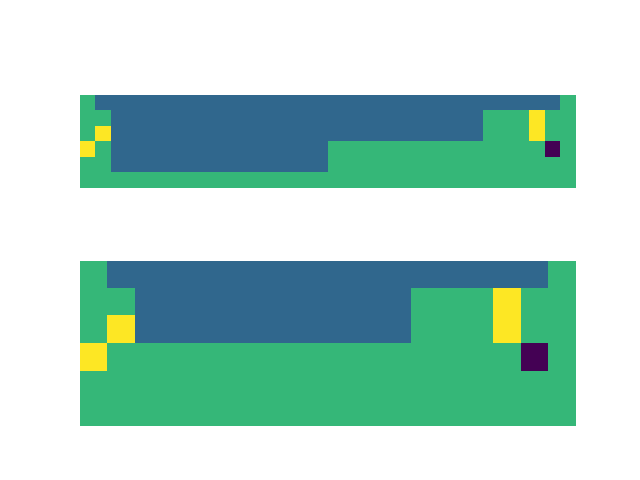
\includegraphics[width=\linewidth]{ex1TPR.png}
	\caption{Representaci\'on de la tabla peri\'odica generada con los m\'etodos de la secci\'on \ref{sec:variantes}. (Arriba/abajo) representaci\'on incluyendo/sin serie de lant\'anidos.}
	\label{fig:fig1}
\end{figure}

En la figura \ref{fig:fig1}, ambas representaciones indican que los elementos K, Mg, O, S comparten una composici\'on R-X$_n$ en com\'un, esto es, el compuesto RX$_n$ existe en el conjunto de datos con X = K, Mg, O, S. Adicionalmente se indica la pregunta: Existe el compuesto R-Br$_n$? Como ya se mencion\'o, esto debe ir acompa\~nado de una etiqueta que marca la respuesta real a esta pregunta, nuevamente basado en el conjunto de datos. Esto convierte la tarea de leer la tabla peri\'odica en una tarea de aprendizaje supervisado.

Al analizar los resultados de esta prueba, se encuentran similaridades entre, por ejemplo, el H y K debido a su presencia en los compuestos $\ce{H2O}$ y $\ce{KOH}$ (bajo el segundo m\'etodo), adem\'as de la ya mencionada en el sistema con Br y Cl, entre otros. Esto sugiere que es el m\'etodo m\'as apropiado. En general se encuentran similitudes con sentido (desde lo que se ense\~na comunmente sobre la TP), adem\'as de esto se espera que las similitudes ''raras" sean suprimidas estad\'isticamente, esto es, si la similitud es demasiado extra\~na entonces ocurre muy pocas veces y otras similitudes m\'as comunes sobresalen.
Esto puede ser una ventaja o una desventaja seg\'un el contexto, sin embargo esto podr\'ia evaluarse despu\'es de obtener los primeros modelos.

\subsection{Ideas para sistema predictor}
La idea inicialmente es utilizar redes neuronales para aproximar la funci\'on descrita por la ecuaci\'on \ref{eq:eq1}. La arquitectura a usar es uno de los grandes problemas debido a que no existe una \'unica manera de obtener una \'optima y usualmente se hace uso del ensayo y error. Adicionalmente en las arquitecturas convencionales existen limitaciones en t\'erminos del tipo de datos que pueden usarse, por lo que esto debe pensarse detenidamente. Por ejemplo, las redes convolucionales (CNN) se usan para la lectura de im\'agenes, estas im\'agenes deben tener un tama\~no fijo, lo cual no es un problema en nuestro caso pues la tabla peri\'odica tiene un tama\~no (en pixeles) igual para todas las im\'agenes.

Un problema de nuestra representaci\'on, sin embargo, es que no conserva nada de la informaci\'on del fragmento R ni del sub\'indice n, sino s\'olo de los elementos que se combinan con R en la proporci\'on n. Esto puede resultar problem\'atico sobre todo en la aplicaci\'on de estimaci\'on de propiedades de nuevos compuestos. Esto es claro en el siguiente ejemplo: el compuesto $\ce{C6H5-Cl}$ es un clorobenceno, y claramente puede prepararse un an\'alogo con Br y I. En este caso R es $\ce{C6H5}$. Similarmente ocurre con NaCl, donde se pueden tambi\'en formar NaBr y NaI. Claramente los Rs son muy diferentes, as\'i como los compuestos formados por estos, de manera que no puede pretenderse obtener propiedades de los compuestos \'unicamente a partir de la representaci\'on hasta aqu\'i formulada.

Una soluci\'on puede ser convertir este R en un vector, donde cada entrada indica la cantidad de equivalentes de un elemento que se encuentran en este R, y su longitud es la cantidad de elementos \'unicos en el dataset. El problema de esto es que no es compatible con la arquitectura de una CNN.

Esto puede arreglarse creando una nueva arquitectura de manera que permita ambas representaciones simult\'aneamente. En esta arquitectura, se lee por un lado la representaci\'on en tabla peri\'odica mediante capas convolucionales, y por el otro el vector R por medio de redes neuronales densas (DNN) convencionales. Estas dos arquitecturas generan cada una un vector, que puede concatenarse para generar una \'unica entrada a una s\'ola red, que producir\'a la salida esperada, sea probabilidad de existencia o propiedades de compuestos, etc. Esto es similar a lo que se muestra en \cite{parallelNN}, donde se presenta un concepto similar (figura \ref{fig:fig2}). En nuestro caso, sin embargo, uno de los ''caminos''  paralelos ser\'ia una CNN que recibe la representaci\'on de tabla peri\'odica aqu\'i propuesta, mientras que el otro ser\'ia una DNN que recibe informaci\'on sobre el fragmento R correspondiente.

\begin{center}
\begin{figure}[h!]
	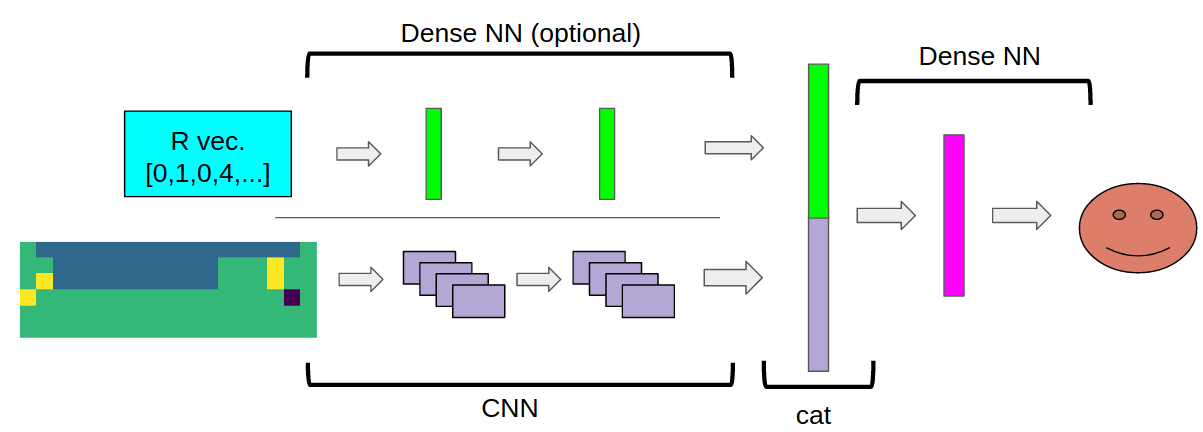
\includegraphics[width=7cm]{CDDNN.png}
	\caption{Arquitectura propuesta de red neuronal. Imagen obtenida de \cite{parallelNN}.}
	\label{fig:fig2}
\end{figure}
\end{center}






\renewcommand\refname{Referencias}
\bibliography{bib}
\bibliographystyle{ieeetr}

\end{document}             % End of document.

